%!TEX program = xelatex 
\documentclass{standalone}%opcao draft remove os links
\usepackage{amssymb,amsmath,amsfonts,amsthm,amstext,pxfonts}
\usepackage{graphicx}
\usepackage[usenames,dvipsnames]{xcolor}
\usepackage{subfigure}
\usepackage{tikz,tikz-3dplot,tkz-euclide,circuitikz,siunitx,pstricks-add,pst-coil,pst-3dplot}
\usepackage{pst-plot,pst-func,pst-eucl,pst-solides3d}
\usetkzobj{all}
\usetikzlibrary{scopes}
\usetikzlibrary{through}
\usetikzlibrary{lindenmayersystems}
\usetikzlibrary[shadings]
\usetikzlibrary{arrows}
\usetikzlibrary{intersections,positioning}


\begin{document}
    \pagenumbering{gobble}
    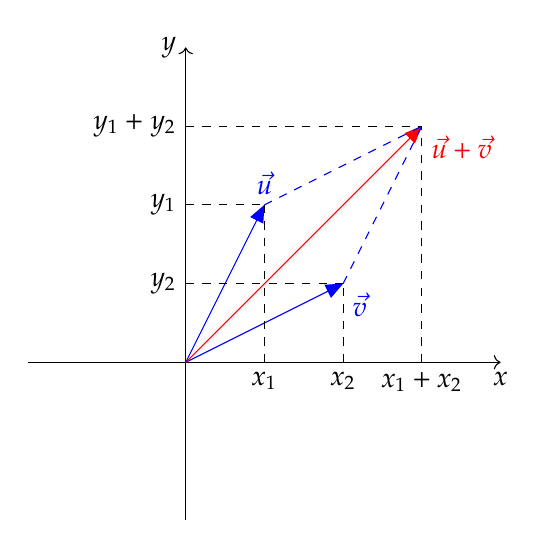
\begin{tikzpicture}[scale=2]%soma de vetores no plano
        \coordinate (A) at (0,0);
        \coordinate (V) at (0.5,1);
        \coordinate (W) at (1,0.5);
        \coordinate (B) at (0,1);
        \coordinate (VW) at ($(V)+(W)$);
        %defini\c{c}\~ao das coordenadas dos eixos cartesianos
        \coordinate (F) at (-1,0);
        \coordinate (G) at (0,-1);
        \coordinate (X) at (2,0);
        \coordinate (Y) at (0,2);
        % Styles
        \tikzstyle{axes}=[]

        \begin{scope}[style=axes]%constr\'oi os eixos cartesianos
            \draw[->] (F) -- (X) node[below] {$x$} coordinate(x axis);
            \draw[->] (G) -- (Y) node[left] {$y$} coordinate(y axis);
        \end{scope}

        \draw[->,>=triangle 45,color=blue] (A)--(V)
          node[above]{$\vec{u}$};
        \draw[->,>=triangle 45,color=blue] (A)--(W)
          node[below right]{$\vec{v}$};
        \draw[->,>=triangle 45,color=red] (A)--(VW)
          node[below right]{$\vec{u}+\vec{v}$};
        \draw[dashed,>=triangle 45,color=blue] (V)--(VW);
        \draw[dashed,>=triangle 45,color=blue] (W)--(VW);
        \draw[dashed,color=black] let \p1 = (V) in (\x1,0) -- (\x1,\y1)
          node[at start, below]{$x_1$};
        \draw[dashed,color=black] let \p1 = (V) in (0,\y1) -- (\x1,\y1)
          node[at start, left]{$y_1$};
        \draw[dashed,color=black] let \p1 = (W) in (\x1,0) -- (\x1,\y1)
          node[at start, below]{$x_2$};
        \draw[dashed,color=black] let \p1 = (W) in (0,\y1) -- (\x1,\y1)
          node[at start, left]{$y_2$};
        \draw[dashed,color=black] let \p1 = (VW) in (\x1,0) -- (\x1,\y1)
          node[at start, below]{$x_1 + x_2$};
        \draw[dashed,color=black] let \p1 = (VW) in (0,\y1) -- (\x1,\y1)
          node[at start, left]{$y_1 + y_2$};
    \end{tikzpicture}
\end{document}